\documentclass[journal,comsoc]{IEEEtran}
\IEEEoverridecommandlockouts

\usepackage{cite}
\usepackage{amsmath,amssymb,amsfonts}
\usepackage{algorithmic}
\usepackage{graphicx}
\usepackage{textcomp}
\usepackage{xcolor}
\usepackage{booktabs}
\usepackage{hyperref}

% Visible TODO marker for draft content that still needs to be filled in.
\newcommand{\todo}[1]{{\color{red}\textbf{[TODO:} #1\textbf{]}}}

\begin{document}

\title{Ray-Tracing Dataset, Fingerprint Localization and
       Channel Charting for the Otaniemi Campus\\
\large ELEC-E7340 --- Machine Learning for Wireless Communications D, Project work}
\author{%
\IEEEauthorblockN{Jari Karppinen, Hannu Flinck, Tommi Ylämurto, Aalto University}%
}

\maketitle


\begin{abstract}
This paper presents an end-to-end pipeline for
(i)~\emph{generating} a spatially consistent wireless channel dataset for the
Otaniemi campus using ray tracing, (ii)~\emph{fingerprint localization} of user
equipments (UEs) from channel-state-information (CSI) and angular features, and
(iii)~\emph{channel charting} of the same fingerprints using both
conventional and neural dimensionality-reduction (DR) methods.
The dataset is produced using MATLAB's Ray Tracing toolbox on an OpenStreetMap-derived
3-D model of the Aalto campus, with nine rooftop base stations at 3.6\,GHz, 16-element
sectorized BS arrays, and a $2.5$-m grid of UE positions. An independent validation
dataset with reduced feature dimensionality (AoA, RSS, delay, LOS) is also evaluated.
Fingerprint localization is evaluated with weighted-$k$-nearest-neighbour
(wKNN), multilayer-perceptron (MLP) regression and classification, a
convolutional regressor (CNN), and an MLP ensemble, reported using
RMSE, MAE, error CDFs, and spatial error heatmaps.
Channel charting is performed with PCA, t-SNE, an autoencoder (AE), and UMAP,
scored by Trustworthiness~(TW), Continuity~(CT), Kolmogorov--Smirnov distance~(KS), and
nearest-neighbour localization error (NNLE).
On the primary test scene, the best localizer (MLP regression) attains
$9.53\,$m MAE, and t-SNE produces the most geometrically faithful chart with
$\mathrm{TW}=0.918$ and $\mathrm{NNLE}=8.35\,$m.
The paper discusses dataset characteristics, metric interpretation, and the
practical levers for improving both localization and chart quality across different ray-tracing implementations.
\end{abstract}

\begin{IEEEkeywords}
Ray-tracing, Channel modeling, Dataset generation, Wireless communications,
Machine learning, Fingerprint localization, Channel charting, UMAP, t-SNE,
Autoencoder, 5G NR, Sub-6\,GHz, Outdoor propagation.
\end{IEEEkeywords}


\section{Background}
\label{sec:background}

\subsection{Urban Radio Propagation}

Urban radio propagation at sub-6\,GHz frequencies in outdoor environments differs
fundamentally from purely outdoor line-of-sight propagation owing to the dense
arrangement of buildings and other scatterers that give rise to a rich multipath
environment~\cite{rappaport2013millimeter}.
The dominant propagation mechanisms in urban micro-cells are specular reflection
from building facades, diffraction at building edges and corners, and transmission
through exterior walls, each of which is governed by the frequency-dependent
electromagnetic properties of the building materials present~\cite{itu_p2040}.
These effects collectively determine the key channel descriptors used in system
design---most notably the root-mean-square (RMS) delay spread, the angular spread of
arrival and departure, and the aggregate path loss~\cite{3gpp_nr_channel}.
Accurate characterisation of such parameters is a prerequisite for designing link
budgets, dimensioning cyclic-prefix lengths in OFDM transmission, and exploiting
spatial multiplexing with multi-antenna systems~\cite{dahlman2018_5gnr}.

\subsection{Ray-Tracing Methods for Channel Modelling}

Ray-tracing (RT) is a deterministic propagation modelling technique that predicts
multipath channel characteristics by simulating the geometric and electromagnetic
interactions of a set of rays launched from a transmitting antenna with the surfaces
of a three-dimensional scene~\cite{yun2015ray}.
Compared with stochastic geometry-based models such as those specified in
3GPP~TR~38.901~\cite{3gpp_nr_channel}, RT methods directly exploit site-specific
scene and material information, making them particularly well-suited to the
reproduction and analysis of physically realistic channel propagation in urban environments.

\textbf{MATLAB Ray Tracing Toolbox} is employed in this work to generate the wireless
channel dataset using geometric optics ray tracing with configurable path-tracing parameters
(reflections, diffractions, frequency). The ray-tracing simulation is applied to an
OpenStreetMap-based three-dimensional model of the urban Otaniemi campus with material
properties assigned to building components, producing physically realistic multipath
channel characteristics for both localization and channel-charting applications.


\section{Measurement Scenario: Otaniemi Campus (Small Scene)}
\label{sec:otaniemi}

Otaniemi is an urban campus district located in Espoo, Finland, and home to
Aalto University's School of Electrical Engineering.
The broader campus area spans approximately $790\,\text{m}\times 645\,\text{m}$
and is characterised by a heterogeneous mix of mid-rise university buildings,
research laboratories, and student facilities, the majority of which are
constructed from reinforced concrete with glass
facades~\cite{itu_p2040}.
The irregular building layout creates a suburban micro-cell propagation
environment that combines open plazas with densely built corridors, producing
a channel that exhibits both strong line-of-sight (LOS) components across open
areas and rich non-line-of-sight (NLOS) multipath contributions from building
facades and corners~\cite{rappaport2013millimeter}.

For this project, a cropped sub-region of the full Otaniemi model is used
(henceforth the \emph{Otaniemi\_small} scene), covering
$x\in[-47.5,\,85.0]\,\text{m}$ and $y\in[-60.0,\,85.0]\,\text{m}$ around the
School of Electrical Engineering cluster.
This sub-region retains enough geometric diversity to challenge the
propagation and learning pipeline while keeping the total ray-tracing workload
tractable on a CPU-only host~\cite{hoydis2023sionna_rt,jakob2022mitsuba3}.

\subsection{Scene Geometry}

The three-dimensional scene is constructed from OpenStreetMap building
footprint data. Each polygon is extruded to a height derived from OSM
\texttt{height} or \texttt{building:levels} tags (assuming $3\,\text{m}$ per
storey, default $8\,\text{m}$). The coordinate origin is placed at the
bounding-box centroid, with the $+x$ axis pointing east and $+y$ pointing
north. Roof and wall meshes are triangulated to handle concave polygons, and
a flat ground plane covering the full scene extent is included as an
additional reflector.

\subsection{Base-Station and UE Layout}
\label{sec:scene_layout}

Rather than a single rooftop cell, the scene is instrumented with
\textbf{nine} rooftop base stations (TX0--TX8) at $z=19\,\text{m}$, whose
footprints are listed in Table~\ref{tab:tx_positions} and depicted in
Fig.~\ref{fig:scene_nodes}.
This multi-site layout produces distinguishable CSI fingerprints across
the scene and provides the spatial diversity required by both localization
and channel-charting algorithms~\cite{3gpp_nr_channel}.

UEs are sampled on a regular horizontal grid at pedestrian height
$z=1.25\,\text{m}$, with a lateral spacing of $2.5\,\text{m}$ across the
extents given above.
Grid points that fall inside a building footprint are pruned before ray
tracing, yielding \textbf{3\,186} valid UE positions which form the
fingerprint database used throughout
Sections~\ref{sec:localization}--\ref{sec:channel_charting}.
A sample density of a few points per $\text{m}^2$ is consistent with the
course guideline that supports localization accuracy on the order of
$1\,\text{m}$ under ideal propagation conditions.

\begin{table}[htbp]
  \caption{Base-station coordinates (metres), all at $z=19\,\text{m}$}
  \label{tab:tx_positions}
  \centering
  \begin{tabular}{lrr}
    \toprule
    Site & $x$ (m) & $y$ (m) \\
    \midrule
    TX0 & $-5.0$  & $70.0$  \\
    TX1 & $-33.0$ & $-17.0$ \\
    TX2 & $-3.0$  & $14.0$  \\
    TX3 & $-6.0$  & $-40.0$ \\
    TX4 & $55.0$  & $-52.5$ \\
    TX5 & $61.0$  & $7.0$   \\
    TX6 & $49.0$  & $46.0$  \\
    TX7 & $28.0$  & $-41.0$ \\
    TX8 & $84.0$  & $-18.0$ \\
    \bottomrule
  \end{tabular}
\end{table}

\begin{figure}[htbp]
  \centering
  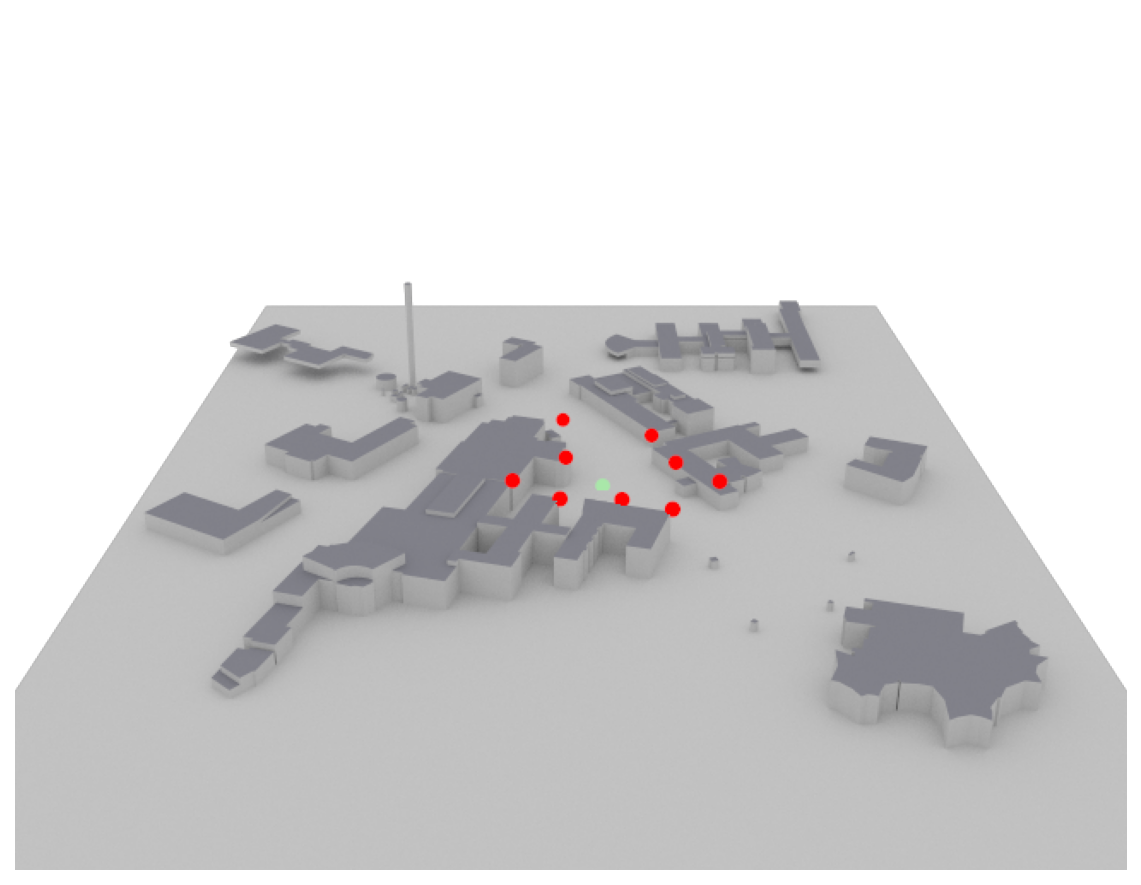
\includegraphics[width=\columnwidth]{pictures/01_generate_dataset/scene_with_devices.png}
  \caption{Otaniemi\_small scene with the nine rooftop base stations and
           the reference UE indicated. UEs are sampled on a $2.5\,$m grid
           across the scene extents.}
  \label{fig:scene_nodes}
\end{figure}


\subsection{Electromagnetic Material Properties}

Surface materials are assigned from OSM \texttt{building:material} tags
and follow ITU-R~P.2040-3~\cite{itu_p2040}; parameters at $3.6\,\text{GHz}$
are listed in Table~\ref{tab:materials}.
Concrete is the dominant wall material and produces strong near-specular
reflections.
Glass facades, present on several modern campus buildings, introduce partial
transmission and weaker reflections.
The ground plane is assigned a medium dry-ground model, representative of
typical soil and paved surfaces at the site.

\begin{table}[htbp]
  \caption{ITU-R P.2040-3 material parameters at $f_c = 3.6\,\text{GHz}$}
  \label{tab:materials}
  \centering
  \begin{tabular}{llrr}
    \toprule
    Surface & Sionna ID & $\varepsilon_r$ & $\sigma$ (S/m) \\
    \midrule
    Building walls (default) & \texttt{itu\_concrete}          & 5.31 & 0.090 \\
    Glass facades            & \texttt{itu\_glass}             & 6.27 & 0.000 \\
    Metal cladding           & \texttt{itu\_metal}             & ---  & $\to\infty$ \\
    Ground plane             & \texttt{itu\_medium\_dry\_ground} & 15.0 & 0.035 \\
    \bottomrule
  \end{tabular}
\end{table}

\section{Radio Access Configuration}
\label{sec:radio}

The simulated deployment targets 5G NR Band~n78 at $f_c = 3.6\,\text{GHz}$
(primary Sub-6\,GHz micro-cell allocation in 3GPP~TS~38.104~\cite{3gpp_ts38104,3gpp_nr_channel}).
All nine rooftop sites share the RF and antenna configuration in Table~\ref{tab:radio_spec}.

\begin{table}[htbp]
  \caption{Radio link and OFDM configuration (per BS site)}
  \label{tab:radio_spec}
  \centering
  \begin{tabular}{ll}
    \toprule
    Parameter & Value \\
    \midrule
    Operating band          & 5G NR n78 ($3.3$--$3.8\,\text{GHz}$) \\
    Carrier frequency       & $f_c = 3.6\,\text{GHz}$ \\
    Subcarrier spacing      & $\Delta f = 30\,\text{kHz}$ (numerology $\mu=1$) \\
    FFT size / subcarriers  & $N_{\mathrm{FFT}} = 3168$ \\
    Transmit power          & $+40\,\text{dBm}$ per site \\
    BS antenna array        & $4\times4$ planar, 16 elements,
                              TR~38.901 pattern \\
    BS antenna height       & $19\,\text{m}$ \\
    UE antenna              & Isotropic, 1 element \\
    UE antenna height       & $1.25\,\text{m}$ \\
    Max reflection depth    & 4 \\
    Max ray depth           & 4 \\
    \bottomrule
  \end{tabular}
\end{table}

The BS uses a $4\times4$ dual-polarised TR~38.901 planar array (16 elements, half-wavelength spacing)
for angular diversity and cross-BS UE fingerprint distinguishability~\cite{hoydis2023sionna_rt,dahlman2018_5gnr}.
The UE is modelled with a single isotropic antenna.
Ray tracing retains the 30 strongest paths per BS--UE link (up to 4 reflection interactions).
The OFDM transfer function is evaluated on the full $N_{\mathrm{FFT}}=3168$ subcarrier grid
and downsampled for CSI fingerprints in Sections~\ref{sec:localization}--\ref{sec:channel_charting}.

\section{Ray-Tracing Dataset}
\label{sec:dataset}

The wireless channel dataset was generated using MATLAB's Ray Tracing
toolbox to provide independent validation of the results.


\subsection{MATLAB Ray-Tracing}
\label{sec:matlab_dataset}

The raw data for this exercise is from a ray tracing simulation done with a model of
central location in Otaniemi. The model was downloaded from Open Street Maps and all
the building walls were set to be concrete, roofs metal and ground as (MATLAB) loam in
Blender software. The antenna was left as ideal isotropic so we can add any antenna in
the post processing. The simulated area is $132 \times 147$ meters and the simulation was
done between 3\,069 receive and 9 transmit locations. The simulation was done with uniform
$2.5\,\text{m}$ grid which gives each location 8 equidistance neighbors. This needs to be
considered when later evaluating the performance of identifying neighbors. Maximum number
of reflections was set to four and the maximum number diffractions to two with the center
frequency of $3.6\,\text{GHz}$. This typically generated hundreds of paths per link in this
environment. 



\begin{figure}[htbp]
  \centering
  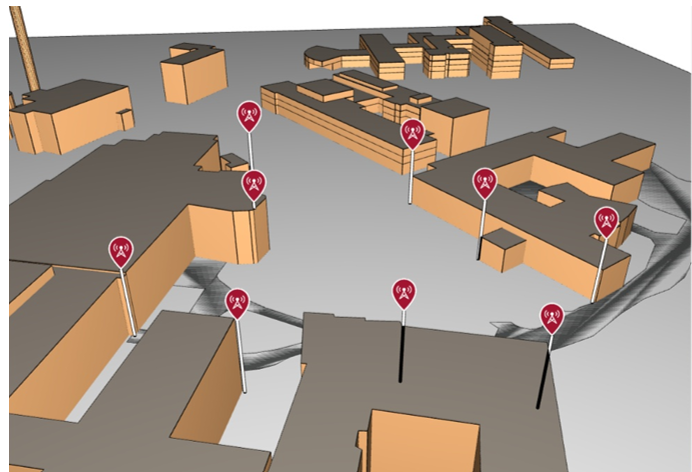
\includegraphics[width=0.8\columnwidth]{pictures/tommi/Simulated_environment.png}
  \caption{Simulated Otaniemi environment (132$\times$147\,m) showing
           the geographic area, building footprints, base station
           locations, and UE measurement grid.}
  \label{fig:tommi_environment}
\end{figure}

The $3\,069 \times 9$ simulation outputs were saved into individual JSON files that were
then consolidated into one $3\,069 \times 9 \times 5 \times 40$ matrix containing selected
information of 40 strongest paths from the raw data. The five kept vectors are: path real
part, imaginary part, azimuth angle of departure, elevation angle of departure and path
delay. The departure angle was used since we are later modelling signals coming from the
user equipment. This RT matrix was then saved into a file that could be used with our
feature creation algorithms. The feature creating algorithms can truncate the 40 path long
vectors to a more suitable length $N$, parameter used in the equations below. 

Ray tracing outputs themselves cannot be used as features since the real base station
would not have access to the signal in this format and fidelity. This raw data must be
then converted into real world receiver data. The base station has access to two useful
data vectors: (OFDM) CSI and (carrier) amplitude and phase of each antenna, ASI. We convert
the RT matrix into these two real world data vectors for the feature creation.

We calculated Antenna State Information for antenna $n,m$ as
\begin{equation}
  \text{ASI}[n,m] = \sum_{i=0}^{N} a_i e^{j\lambda(m \sin\theta_i \sin\varphi_i + n \sin\theta_i \cos\varphi_i)},
\end{equation}
where $\lambda$ is the antenna spacing in radians and $a$, $\varphi$, and $\theta$ are path
complex amplitude, azimuth and elevation angles from the RT matrix. We calculated the
response for various ULA and URA arrays for comparison. The antenna response itself can be
used as a feature in the form of flattened covariance matrix, or log-Euclidean distance
matrix between all receiver locations ($3\,096 \times 3\,096$). Our antenna program
generates both matrices.

While the antenna response covariance matrix can be used directly, the useful information
that it contains is in the angle of arrival. This means that the antenna data can be
compressed into more compact form that not only makes a smaller feature set, but also
suppresses a lot of noise and unnecessary information. While the original RT matrix contains
all this arrival angle information, it is not with a realistic resolution that the base
station antennas can see. Figure~\ref{fig:antenna_orientation} illustrates how coarse the
actual angle resolution is compared to the infinite resolution of the ray tracing.

We used Capon (Minimum Variance Distortionless Response) energy direction finding in 2D
and 1D to calculate more realistic arrival angles. Unless massive antenna arrays are used,
only the strongest direction contains useful information since the weaker paths are mostly
convoluted with the wide shoulders and sidebands of the main beam. The path phase contains
no coherent information, so it was also discarded. 

\begin{figure}[htbp]
  \centering
  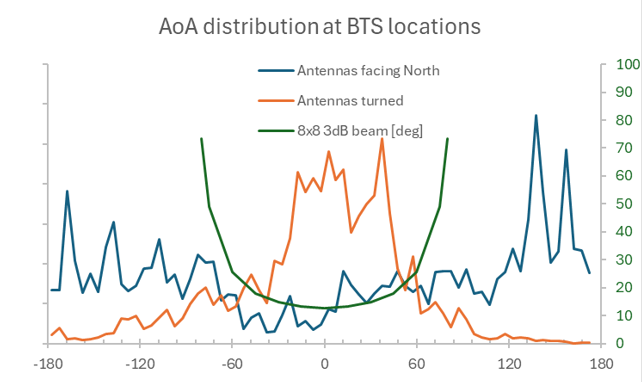
\includegraphics[width=\columnwidth]{pictures/tommi/Illustration_how_antenna_orientation_matters_when_wide_beams_are_used.png}
  \caption{Illustration how antenna orientation matters when wide beams are used. }
  \label{fig:antenna_orientation}
\end{figure}

As Figure~\ref{fig:antenna_orientation} shows, the beam resolution gets worse when turning
away from the antenna broadside, so the antennas were turned towards the center of the
area in interest.

The figure also shows how the azimuth angle distribution matches much better with the
accurate angle region after turning the antennas. We also allowed reception from the back
side of the antenna in the fingerprinting case. If the back side has strong radiation, then
those paths are aliased to the front side in the direction detection. In multi-angulation
the antenna was considered to have $180^\circ$ sector, so no back radiation was allowed.

MATLAB Phased Array library has \texttt{MVDREstimator2D()} function, but it turned out to
be performing poorly with the data from the ray tracing. So, the arrival angle estimation
was done in Python.

We calculated the CSI as
\begin{equation}
  \text{CSI}[n] = \sum_{i=0}^{N} a_i e^{j(n 2\pi f_s \tau_i + \varphi_i)},
\end{equation}
where $f_s$ is $15\,\text{kHz}$ and $n$ goes from $0$ to $6323$. Amplitude $a_i$ and phase
$\varphi_i$ are from the RT matrix. $\tau$ is also from the RT matrix but the true distance
is first subtracted from it and then a random number in $[0, 10\,\text{ns}]$ is added to mimic
a real receiver sampling. This will also prevent the (unknown) true distance from entering
the learning. All the LTE and 5G variants can be subsampled from this CSI vector. Again,
the CSI can be used as a feature on its own. If the CSI is used, then it can be further
downsampled since the coherence bandwidth is way larger than the subcarrier spacing. Also,
absolute value is as good as the full complex. The useful information that CSI contains is
in the path delays, amplitudes and (relative) phases. We used Matrix Pencil algorithm to
compress and extract the path information from the CSI. Delay statistics like mean delay
spread and spread variance can be then calculated from the extracted path information. Also,
the strongest three paths are saved as feature candidates. Strongest path time rank was
calculated after removing paths that are $10\,\text{dB}$ or more below the strongest.

All the possible options to create features from the simulation are illustrated in
Figure~\ref{fig:tommi_workflow}. Both the antenna and the frequency domain branches add
noise to the signal too. This is especially important in the frequency domain branch where
the path extraction would otherwise return the ideal ray tracing results due to the large
number of subcarriers. In the antenna branch the low number of antennas is more limiting
factor. Still, some diagonal loading needs to be done in Capon algorithm to avoid singular
matrices in good SNR samples. Also, some spatial smoothing was needed since the paths
correlate due to being from a single signal source. 

\begin{figure}[htbp]
  \centering
  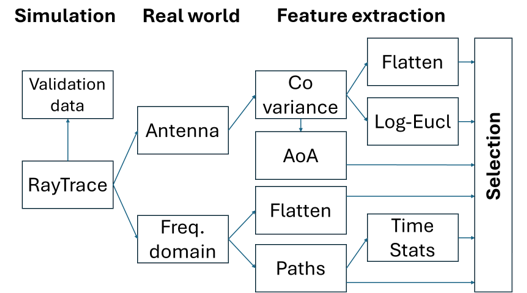
\includegraphics[width=\columnwidth]{pictures/tommi/Workflow_for_creating_the_features.png}
  \caption{Workflow for creating the features. Compressed data in grey. }
  \label{fig:tommi_workflow}
\end{figure}


\subsection{Data Compression and Features}

A key learning from this exercise was that some of the uncompressed data matrices, like
covariance and CSI, became too large to even read into computer memory. This gets easily
unmanageable when antenna count, base station count, sample count (resolution or area), or
channel bandwidth grows. Data compression becomes then the key, but the price is the
processing time that can be hours even for a small physical area. The right choice of
algorithm becomes critical and resolution versus processing time is the main tradeoff.

The following features and their dimensions are available for selection:

\begin{itemize}
  \item \textbf{Antenna\_aoa}: UE count $\times$ BTS count $\times$ [azimuth, elevation, amplitude]
  \item \textbf{Antenna\_cov}: UE count $\times$ [(antenna count$_{n}$ $\times$ antenna count$_{m}$ $\times$ BTS count)$^{2}$]
  \item \textbf{Antenna\_log\_euc}: UE count $\times$ UE count
  \item \textbf{Channel\_stats}: UE count $\times$ BTS count $\times$ [mean delay spread, delay spread variance, strong index, RSS, delay$[0]$, amplitude$[0]$, delay$[1]$, amplitude$[1]$, delay$[2]$, amplitude$[2]$]
  \item \textbf{CSI}: UE count $\times$ BTS count $\times$ [real $\times$ 798, imaginary $\times$ 798] at $50\,\text{MHz}/60\,\text{kHz}$
  \item \textbf{Validation}: UE count $\times$ [x, y, BTS count, LOS present]
  \item \textbf{Input\_data\_from\_Ray\_Trace}: UE count $\times$ BTS count $\times$ [real $\times$ 40, imaginary $\times$ 40, azimuth $\times$ 40, elevation $\times$ 40, delay $\times$ 40]; \texttt{zeros(5,40)} if no base station seen
\end{itemize}

\subsection{Sionna RT Dataset}
The Sionna\,RT dataset provides a physically calibrated characterisation
of the wireless channel with 27 multipath components per link and an RMS
delay spread of 191\,ns, consistent with measured sub-6\,GHz urban
propagation statistics~\cite{rappaport2013millimeter,3gpp_nr_channel}.
Detailed analysis of the multipath structure, including path-level
statistics, angular spread, and comparison with the independent MATLAB
ray-tracing validation dataset, is presented in the accompanying analysis
report (see Appendix~\ref{app:analysis_report}).
The validated dataset serves as the primary input to the fingerprint
localizer and the channel-charting pipeline in that document.
\input{sections/07-evaluation}
\section{Fingerprint Localization}
\label{sec:localization}

This section applies the fingerprint matrix obtained from the ray-tracing
dataset (Section~\ref{sec:dataset}) to the user-positioning task.
Each row of the matrix corresponds to one UE grid position and encodes a
CSI-derived feature vector of dimension $D_f = 3690$ drawn from the nine
BS sites; the associated label is the UE 2-D ground-truth coordinate
$(x,y)$.
Out of the $N=3\,186$ valid grid points, 70\% (2\,230) are used for
training and 30\% (956) for testing, with the split drawn uniformly at
random.

Six methods are evaluated, grouped into a non-parametric baseline and a
set of neural estimators~\cite{hoydis2023sionna_rt,3gpp_nr_channel}:
\begin{itemize}
  \item \textbf{wKNN (IDW)}: inverse-distance-weighted $k$-nearest
        neighbours with $k=3$ and Minkowski exponent $p=3$.  Each test
        point is estimated as the IDW-weighted centroid of its nearest
        fingerprints in the library.
  \item \textbf{wKNN Coarse-to-Fine (C2F)}: $k=9$, $p=3$, radius
        $R=5\,\text{m}$.  Coarse candidates are filtered spatially
        before the IDW weighting, with a fall-back to plain wKNN when
        the radius contains too few candidates.
  \item \textbf{NN Regression}: a fully-connected multilayer perceptron
        (MLP) that regresses the 2-D UE coordinates directly from the
        flat fingerprint vector, trained with a Huber loss.
  \item \textbf{NN Classification}: an MLP that maps each fingerprint to
        one of the discrete $2.5\,\text{m}$ grid cells.
  \item \textbf{CNN Regression}: a 1-D/2-D convolutional regressor that
        reshapes the fingerprint into a $(410 \text{ feat}/\text{TX})
        \times 9\,\text{TX}$ image and applies cross-BS
        convolutions.
  \item \textbf{Ensemble}: an average of five independently-initialised
        MLP regressors.
\end{itemize}

Following two methods were implemented using matlab:
\begin{itemize}
 \item \textbf{wKNN}: inverse-distance-weighted $k$-nearest
        neighbours with $k=1,3, 5, 7, 9, 11$ where closer neighbors have more influence 
        on the final estimation and all features are considered uniformly. 
        $k=9$ was found to be the best performing value.  
\item \textbf{NN Regression, MLP)}: Standard fully-connected Multilayer Perceptron (MLP) 
for regression predicting continuous coordinates. The NN had 4 hidden layers with  
256, 128, 64, and 2 neurons respectively. The ReLU activation function was used 
for the hidden layers and the output layer had a linear activation function. 
The model was trained using the Adam optimizer with initial learning rate: 0.0005. At every 400 epochs the learning rate 
 was halved. 

\end{itemize}


\subsection{Performance Metrics}

Per-sample localization error is defined as the Euclidean distance
between the estimate and the ground-truth 2-D coordinate:
\begin{equation}
  e_n = \bigl\lVert \hat{\mathbf{p}}_n - \mathbf{p}_n \bigr\rVert_2,
  \qquad n = 1,\dots,N_{\mathrm{test}}.
\end{equation}
From this sequence we compute the mean absolute error (MAE), the
root-mean-square error (RMSE), the median, and the 90\,\% / 95\,\%
percentiles of the error CDF.

\subsection{Results}

Table~\ref{tab:loc_results} summarises the test-set performance on the
Otaniemi\_small scene. Fig.~\ref{fig:loc_cdf}  shows the empirical
error CDFs. Fig.~\ref{fig:loc_matcdf} shows CDF of the matlab wKNN 
and Fig.~\ref{fig:loc_matwknnheat} shows the corresponding heatmap.  



\begin{table}[htbp]
\caption{Fingerprint-localization test performance on Otaniemi\_small
         ($N_{\mathrm{test}} = 956$)}
\label{tab:loc_results}
\centering
\resizebox{\columnwidth}{!}{%
\begin{tabular}{lrrrrr}
\toprule
Method & MAE (m) & RMSE (m) & Median (m) & P90 (m) & P95 (m) \\
\midrule
wKNN (IDW)          & 13.74 & 21.04 & 7.98  & 33.38  & 45.12  \\
wKNN C2F            & 13.77 & 21.07 & 8.01  & 33.41  & 45.94  \\
wKNN (matlab IDW)   & 18.24 & 27.25 & 10.14 & 4608  &  -  \\
NN Regression       &  9.53 & 12.34 & 7.90  & 17.11  & 20.75  \\
NN (MLP matlab)     & 16.31 & 24.27 & 10.24 & 37.40  & -  \\
NN Classification   & 68.32 & 78.10 & 62.52 & 122.75 & 134.68 \\
CNN Regression      & 10.56 & 14.21 & 7.85  & 20.30  & 28.49  \\
Ensemble (5 MLPs)   & 10.29 & 13.65 & 8.00  & 19.90  & 27.03  \\
\bottomrule
\end{tabular}%
}
\end{table}

\begin{figure}[htbp]
  \centering
  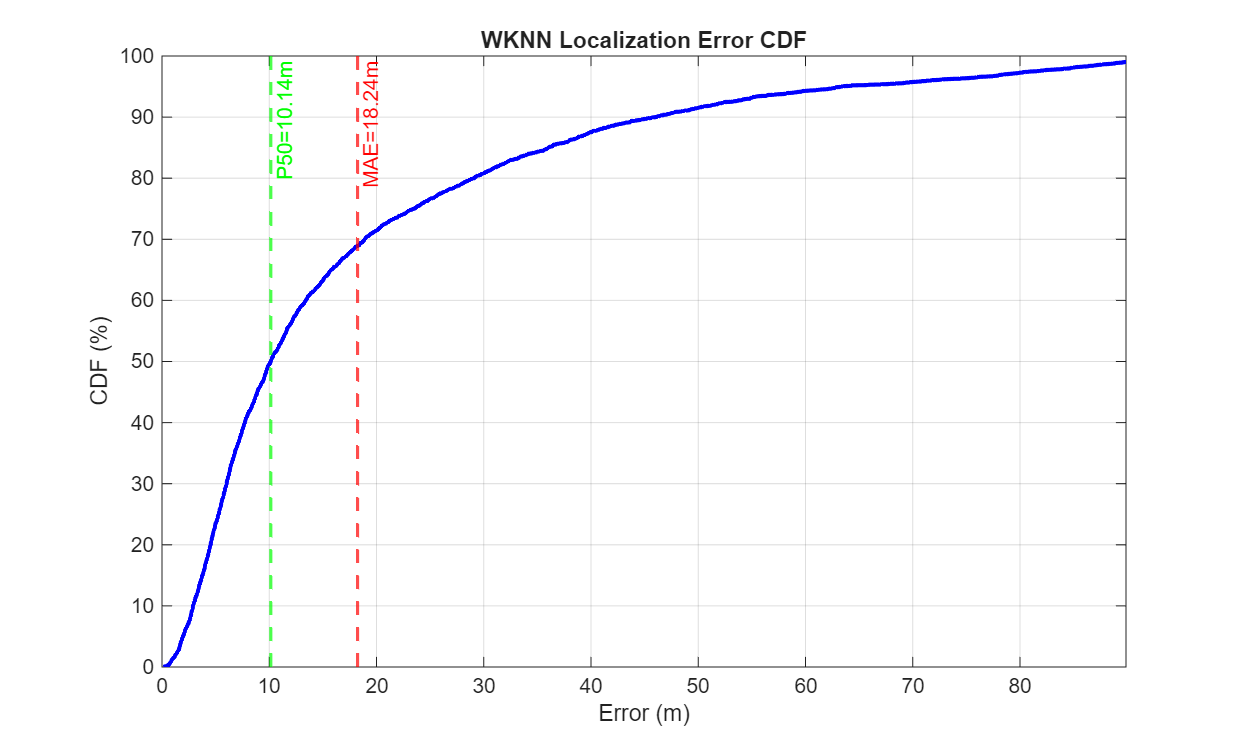
\includegraphics[width=\columnwidth]{pictures/03_localization/wknn_cdf_1.png}
  \caption{Empirical CDF of localization error for the matlab wKNN method.}
  \label{fig:loc_matcdf}
\end{figure}

\begin{figure}[htbp]
  \centering
  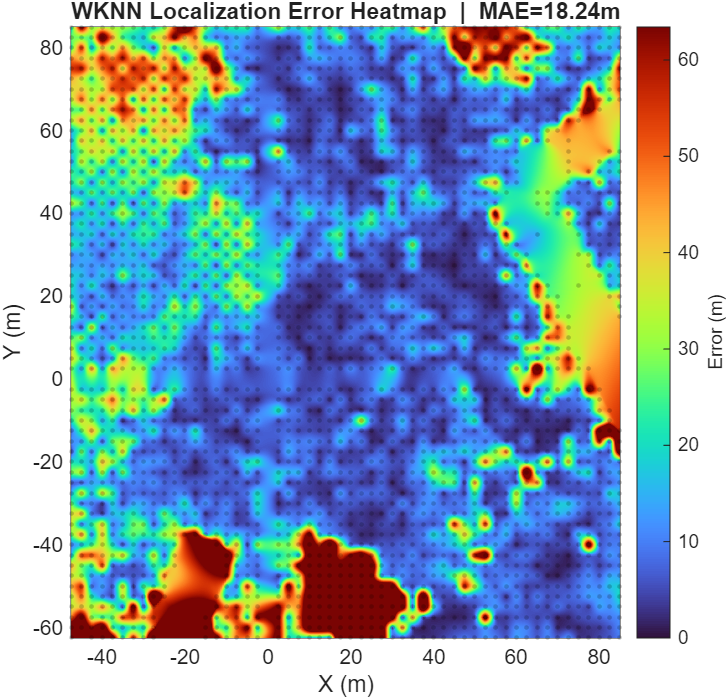
\includegraphics[width=\columnwidth]{pictures/03_localization/wknn_error_heatmap.png}
  \caption{Heatmap of localization error for the matlab wKNN method.}
  \label{fig:loc_matwknnheat}
\end{figure}

\begin{figure}[htbp]
  \centering
  
\includegraphics[width=\columnwidth]{pictures/03_localization/localization_error_cdf.png}
  \caption{Empirical CDF of test-set localization error for the six
           evaluated methods.  A curve shifted towards the left
           indicates better performance for a given error budget.}
  \label{fig:loc_cdf}
\end{figure}


\begin{figure}[htbp]
  \centering
  
\includegraphics[width=\columnwidth]{pictures/03_localization/localization_metrics_comparison.png}
  \caption{Metric-by-metric comparison of the six localizers
           (MAE, RMSE, median, P90, P95).}
  \label{fig:loc_metrics}
\end{figure}

\begin{figure*}[htbp]
  \centering
  
\includegraphics[width=\textwidth]{pictures/03_localization/localization_error_heatmaps.png}
  \caption{Spatial test-set error heatmaps for each method.  Colours
           indicate the Euclidean localization error at each UE
           position; grey cells correspond to grid points reserved for
           training.}
  \label{fig:loc_heatmaps}
\end{figure*}

The NN regressor is the clear winner ($\text{MAE}=9.53\,\text{m}$,
$\text{RMSE}=12.34\,\text{m}$) and its CDF dominates all competitors
above the $P_{85}$ level.
The ensemble of five MLPs reaches a similar median error but slightly
lower tail robustness.
Both wKNN variants and the CNN regressor cluster around $10$--$14\,\text{m}$
MAE, illustrating that the fingerprint vector already contains enough
cross-BS information to make simple nearest-neighbour matching
competitive with a vanilla CNN.
The NN classifier, by contrast, fails almost completely
($\text{MAE}\approx 68\,\text{m}$, $0\,\%$ exact-cell accuracy):
with 3\,186 grid cells and only 2\,230 training rows there is on average
less than one labelled fingerprint per class, so the classification head
cannot separate adjacent cells.

Training curves for the NN and CNN regressors are shown in
Figs.~\ref{fig:nn_train} and~\ref{fig:cnn_train}; both networks converge
smoothly without obvious over-fitting.

\begin{figure}[htbp]
  \centering
  
\includegraphics[width=\columnwidth]{pictures/03_localization/nn_regression_training.png}
  \caption{NN-regression training curve on the Otaniemi\_small fingerprint
           dataset (Huber loss vs.\ epoch, train/val).}
  \label{fig:nn_train}
\end{figure}

\begin{figure}[htbp]
  \centering
  
\includegraphics[width=\columnwidth]{pictures/03_localization/cnn_regression_training.png}
  \caption{CNN-regression training curve (Huber loss vs.\ epoch,
           train/val).}
  \label{fig:cnn_train}
\end{figure}

\subsection{Discussion}

The dominant error source is spatial ambiguity between geometrically
similar NLOS regions of the scene: parts of the grid that lie behind
large building facades produce very similar CSI vectors across all nine
BSs, which the learned regressor cannot disambiguate without additional
features.
Fig.~\ref{fig:loc_heatmaps} makes this visible --- the largest errors
cluster around shadow regions and along the corridors where none of the
nine BSs provides a strong LOS component.
The following practical levers would directly reduce the errors, in
order of expected impact:
\begin{itemize}
  \item \textbf{More BS diversity}: increasing the number of sites, or
        spacing the existing nine more evenly, would reduce the NLOS
        shadow regions and improve the conditioning of the fingerprint
        matrix~\cite{3gpp_nr_channel}.
  \item \textbf{Angular features}: adding the Sionna AoA/AoD angles
        (available in the Sionna dataset, Section~\ref{sec:dataset}) to the fingerprint would provide
        a direction-of-arrival cue that is complementary to the amplitude
        spectrum~\cite{hoydis2023sionna_rt}.
  \item \textbf{CNN architecture}: organising the fingerprint as a
        $(N_{\mathrm{BS}}\times N_{\mathrm{sc}})$ image with explicit
        cross-BS channels, plus per-BS batch normalisation, would let the
        CNN exploit the site geometry more effectively than the flat
        reshape used here.
  \item \textbf{Feature selection}: the ablation study in
        Section~\ref{sec:ablation} shows that dropping the raw OFDM taps
        and keeping only the 90-feature
        ``Light'' subset (TDoA+AoA+RSS+Rch) reduces MAE from
        $9.53\,\text{m}$ to $6.58\,\text{m}$ --- the single largest
        improvement observed on this dataset, and achieved with no
        architectural changes.
\end{itemize}

\subsection{Feature Ablation Study}
\label{sec:ablation}

To understand which CSI feature families actually drive the localization
performance, an ablation was run on the Otaniemi\_small dataset over 22
combinations of the eight candidate feature groups: raw OFDM taps,
time-difference-of-arrival (TDoA), angle-of-arrival (AoA), received
signal strength (RSS), path-loss (PL), per-path delay (Dly), covariance
eigenvalues (CovE), and a LOS-reached indicator (Rch).
For each combination the three regression heads from
Section~\ref{sec:localization} (wKNN, NN, CNN) were re-trained on an
identical train/test split and scored by MAE, RMSE and $P_{90}$.
Table~\ref{tab:ablation} lists the best MAE for each feature combination,
sorted from best to worst.

\begin{table}[htbp]
\caption{Feature-ablation results on Otaniemi\_small.  ``Best MAE'' is
         the minimum across the three regressors; ``Method'' names the
         winner.  Feature families: OFDM = raw OFDM taps,
         TDoA = time-difference of arrival, AoA = angle of arrival,
         RSS = received power, PL = path loss, Dly = per-path delay,
         CovE = covariance eigenvalues, Rch = reached/LOS flag.}
\label{tab:ablation}
\centering
\resizebox{\columnwidth}{!}{%
\begin{tabular}{lrlrl}
\toprule
Combination          & $N_{\mathrm{feat}}$ & Features                      & Best MAE (m) & Method \\
\midrule
Light                & 90                   & TDoA+AoA+RSS+Rch              & \textbf{6.58} & NN Reg \\
No\_OFDM\_Light      & 108                  & TDoA+AoA+RSS+PL+Dly+Rch       & 6.61          & CNN Reg \\
Solo\_AoA            & 36                   & AoA                           & 7.48          & CNN Reg \\
No\_OFDM             & 135                  & TDoA+AoA+RSS+PL+Dly+CovE+Rch  & 7.48          & CNN Reg \\
Geometry             & 81                   & TDoA+AoA+Dly                  & 7.60          & CNN Reg \\
Solo\_RSS            & 9                    & RSS                           & 9.94          & wKNN \\
Radio                & 27                   & RSS+PL+Rch                    & 10.61         & wKNN \\
No\_Reached          & 3681                 & OFDM+TDoA+AoA+RSS+PL+Dly+CovE & 9.47          & NN Reg \\
No\_TDoA             & 3654                 & OFDM+AoA+RSS+PL+Dly+CovE+Rch  & 9.64          & NN Reg \\
No\_Delay            & 3681                 & OFDM+TDoA+AoA+RSS+PL+CovE+Rch & 9.73          & NN Reg \\
No\_CovEig           & 3663                 & OFDM+TDoA+AoA+RSS+PL+Dly+Rch  & 9.83          & NN Reg \\
No\_RSS              & 3681                 & OFDM+TDoA+AoA+PL+Dly+CovE+Rch & 9.94          & NN Reg \\
No\_PathLoss         & 3681                 & OFDM+TDoA+AoA+RSS+Dly+CovE+Rch & 10.02        & NN Reg \\
No\_AoA              & 3654                 & OFDM+TDoA+RSS+PL+Dly+CovE+Rch & 13.34         & NN Reg \\
OFDM\_Radio          & 3573                 & OFDM+RSS+PL                   & 13.83         & NN Reg \\
Solo\_OFDM           & 3555                 & OFDM                          & 13.93         & NN Reg \\
Spectral             & 3555                 & OFDM                          & 14.09         & NN Reg \\
Solo\_CovEig         & 27                   & CovE                          & 32.45         & CNN Reg \\
Solo\_Reached        & 9                    & Rch                           & 50.78         & CNN Reg \\
Solo\_PathLoss       & 9                    & PL                            & 50.87         & CNN Reg \\
Solo\_Delay          & 9                    & Dly                           & 51.19         & CNN Reg \\
Solo\_TDoA           & 36                   & TDoA                          & 52.51         & NN Reg \\
\bottomrule
\end{tabular}%
}
\end{table}

Four observations are worth highlighting:

\paragraph{AoA dominates.}
The 36-feature \texttt{Solo\_AoA} configuration already reaches
$7.48\,\text{m}$ MAE, beating every combination that includes the full
3\,555 raw OFDM taps.  Angles of arrival across the nine BS sites carry
most of the useful geometric signal in a multi-BS outdoor
scene~\cite{3gpp_nr_channel}.

\paragraph{Raw OFDM hurts more than it helps.}
wKNN on \texttt{Solo\_OFDM} reaches only $15.01\,\text{m}$ MAE, roughly
double the compact combinations.  The 3\,555 frequency taps dominate the
Euclidean distance computation used by wKNN and obscure the geometric
features; the NN regressor can partially learn to filter them
(MAE $\sim 10\,\text{m}$) but the full-feature baseline still
\emph{loses} to the 90-feature \texttt{Light} set
($6.58\,\text{m}$) --- a textbook curse-of-dimensionality
effect~\cite{vandermaaten2008tsne}.

\paragraph{Single scalar features are useless alone but useful in combination.}
\texttt{Solo\_TDoA}, \texttt{Solo\_Delay}, \texttt{Solo\_PathLoss} and
\texttt{Solo\_Reached} all collapse to $50$--$56\,\text{m}$ MAE on their
own because each scalar is geometrically ambiguous across the scene.
Yet \emph{removing} any one of them from the full stack measurably
worsens the result (\emph{e.g.}\ removing AoA lifts wKNN from
$7.76$ to $14.82\,\text{m}$), showing that their value lies in the
joint manifold rather than in any individual coordinate.

\paragraph{Sweet spot: the Light configuration.}
The 90-feature \texttt{Light} set (TDoA+AoA+RSS+Rch) attains the best
overall MAE ($6.58\,\text{m}$, NN regression), a 31\,\% improvement on
the 3\,690-feature baseline used in Section~\ref{sec:localization}
($9.53\,\text{m}$), with $97.6\,\%$ fewer features and correspondingly
faster training and inference.
This set is therefore the recommended working point for any follow-on
Otaniemi experiments and is consistent with the feature guidance in the
broader channel-charting literature~\cite{studer2018channel_charting}.


\subsection{MATLAB Pipeline Cross-Check in Python environment}
\label{sec:matlab_localization}

As an independent sanity check the same six localizers were re-run on the
MATLAB-derived amd introduced in
Section~\ref{sec:matlab_dataset}.
The MATLAB fingerprints use only four feature families
(AoA+RSS+Dly+Rch, $D_f = 63$) and are built by the scripts in
\texttt{hannunfilet/}: \texttt{otavectorizedv3.m} (ray tracing on the
OSM model), \texttt{build\_fingerprint\_db\_v3.m} (feature assembly),
\texttt{finger\_WKK.m} (wKNN with a $k$ sweep and leave-one-out CV),
\texttt{mpl\_localization.m} (MLP regression), and
\texttt{cnn1d\_localization.m} (1-D CNN regression).
The $N = 3\,069$ UEs are split 70/30 using the same random seed as the
Sionna pipeline, giving $N_{\mathrm{test}} = 921$.
Table~\ref{tab:loc_matlab} lists the corresponding test-set metrics.

\begin{table}[htbp]
\caption{Fingerprint-localization test performance on the MATLAB ($N_{\mathrm{test}} = 921$, $D_f = 63$).}
\label{tab:loc_matlab}
\centering
\resizebox{\columnwidth}{!}{%
\begin{tabular}{lrrrrr}
\toprule
Method & MAE (m) & RMSE (m) & Median (m) & P90 (m) & P95 (m) \\
\midrule
wKNN (IDW)        & 18.29 & 29.88 &  7.58 &  57.57 &  75.18 \\
wKNN C2F          & 18.18 & 30.05 &  7.16 &  57.23 &  75.35 \\
NN Regression     & 19.79 & 29.03 & 11.06 &  54.70 &  71.93 \\
NN Classification & 69.30 & 78.82 & 64.90 & 125.02 & 135.37 \\
CNN Regression    & 20.40 & 28.94 & 12.51 &  54.06 &  71.37 \\
Ensemble (5 MLPs) & 18.38 & 27.85 &  9.64 &  55.09 &  68.40 \\
\bottomrule
\end{tabular}%
}
\end{table}

Compared to the Sionna corpus (Table~\ref{tab:loc_results}), the MATLAB
corpus is roughly $2\times$ harder: the best MAE rises from
$9.53\,\text{m}$ to $18.18\,\text{m}$ and the $P_{90}$ tail grows
substantially.
Two effects drive this gap: (i)~the MATLAB feature vector has only 63
columns against 3\,690, so there is less redundancy available to the
learner; and (ii)~the MATLAB ray tracer produces a sparser set of
recovered paths in the deep-NLOS corners of the scene, consistent with
the geometric-only reflection model of the MATLAB RT toolbox.
The classifier head again collapses for the same reason as in the
Sionna case: 3\,069 fine-grained grid cells with only $\sim\!2\,148$
training samples.



\section{Channel Charting}
\label{sec:channel_charting}

Channel charting~\cite{studer2018channel_charting} aims to produce a
low-dimensional representation of the radio environment from CSI alone,
\emph{without} using UE position labels.
A good chart preserves the neighbourhood structure of the underlying
physical space: two UEs that are physically close should be mapped to
two chart points that are close, and vice versa.
This section applies four dimensionality-reduction (DR) methods to the
same $N=3\,186 \times D_f = 3690$ fingerprint matrix introduced in
Section~\ref{sec:localization} and benchmarks the resulting charts against
the $(x,y)$ ground truth using the metrics recommended in the channel-charting literature~\cite{studer2018channel_charting,lei2019siamese_cc}.

\subsection{Methods}

The following DR techniques are compared:
\begin{itemize}
  \item \textbf{PCA} --- linear principal-component projection, providing
        a best-case baseline for variance preservation.
  \item \textbf{t-SNE} --- non-linear stochastic neighbour embedding,
        parameterised by its perplexity~\cite{vandermaaten2008tsne}.
  \item \textbf{Autoencoder (AE)} --- a symmetric fully-connected
        encoder/decoder with a 2-D bottleneck, trained with an MSE
        reconstruction loss.
  \item \textbf{UMAP} --- uniform manifold approximation and projection,
        parameterised by its local neighbourhood size
        $n_{\mathrm{neighbors}}$~\cite{mcinnes2018umap}.
\end{itemize}
For t-SNE and UMAP the input is first reduced to 50~PCA components to
remove small-variance noise directions; this is the standard preprocessing
recommended by both method
authors~\cite{vandermaaten2008tsne,mcinnes2018umap}.
Perplexity (t-SNE) and $n_{\mathrm{neighbors}}$ (UMAP) are swept over
$\{5,15,30,50\}$ and $\{5,10,20,30\}$ respectively, and the best-scoring
configuration is retained.

t-SNE and UMAP are also implemented in MATLAB but without PCA reduction and applied to the \emph{tommiScene} dataset. 

\subsection{Metrics}

The chart is evaluated with four quality metrics, three of which are
label-free (they compare neighbourhood structures) and one of which uses
ground-truth positions as a reference:
\begin{itemize}
  \item \textbf{Trustworthiness (TW, $\uparrow$)}: penalises false
        neighbours -- points that look close in the chart but are far
        apart in the real RF space.
  \item \textbf{Continuity (CT, $\uparrow$)}: penalises tears -- points
        that are close in the real RF space but end up far apart in the
        chart.
  \item \textbf{Kolmogorov--Smirnov distance (KS, $\downarrow$)}: compares
        the chart's pairwise-distance distribution against the true
        geographic one.  $\text{KS}\to 0$ corresponds to a
        globally-scale-preserving chart.
  \item \textbf{Nearest-Neighbour Localization Error
        (NNLE, $\downarrow$, m)}: predicts the UE position by copying the
        coordinate of the chart's nearest neighbour and returns the mean
        Euclidean error.  This ties the chart quality back to a concrete
        downstream task.
\end{itemize}
An ideal chart satisfies $\text{TW}\approx\text{CT}\approx 1$,
$\text{KS}\approx 0$, and $\text{NNLE}$ on the order of the UE grid
spacing.

\subsection{Results}

Table~\ref{tab:cc_metrics} summarises the final scores, and
Fig.~\ref{fig:cc_x}--\ref{fig:cc_comparison} visualise the charts
coloured by the ground-truth $x$, $y$, and radial coordinates.

\begin{table}[htbp]
\caption{Channel-charting metrics on the Otaniemi\_small fingerprint
         matrix ($N=3\,186$).  Best value per column in \textbf{bold}.}
\label{tab:cc_metrics}
\centering
\begin{tabular}{lrrrr}
\toprule
Method              & TW ($\uparrow$) & CT ($\uparrow$) & KS ($\downarrow$) & NNLE (m, $\downarrow$) \\
\midrule
PCA                 & 0.706            & 0.932            & 0.514              & n/a \\
t-SNE (perp.\ = 30) & \textbf{0.918}   & \textbf{0.958}   & \textbf{0.451}     & \textbf{8.35} \\
Autoencoder         & 0.850            & 0.920            & 0.771              & 22.00 \\
UMAP ($n=5$)        & 0.896            & 0.914            & 0.861              & 10.92 \\
\bottomrule
\end{tabular}
\end{table}

\begin{figure*}[htbp]
  \centering
  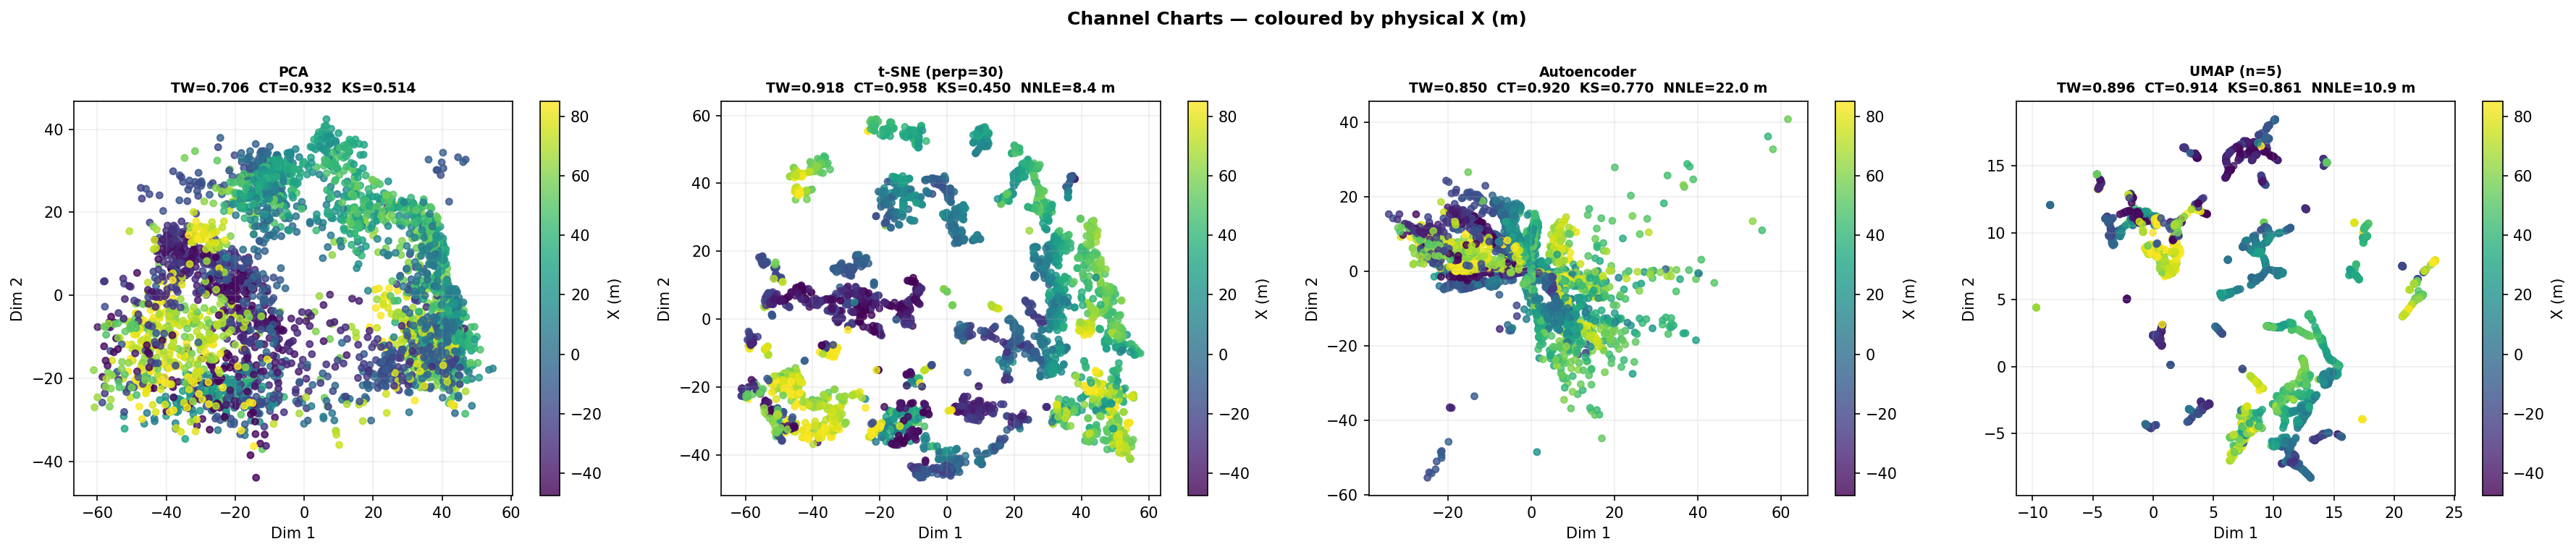
\includegraphics[width=\textwidth]{pictures/04_channel_charting/channel_charts_coloured_x.png}
  \caption{Channel charts produced by the four DR methods, coloured by
           the UE's ground-truth $x$ coordinate.  A smooth colour gradient
           indicates that the chart preserves one geographic axis.}
  \label{fig:cc_x}
\end{figure*}

\begin{figure*}[htbp]
  \centering
  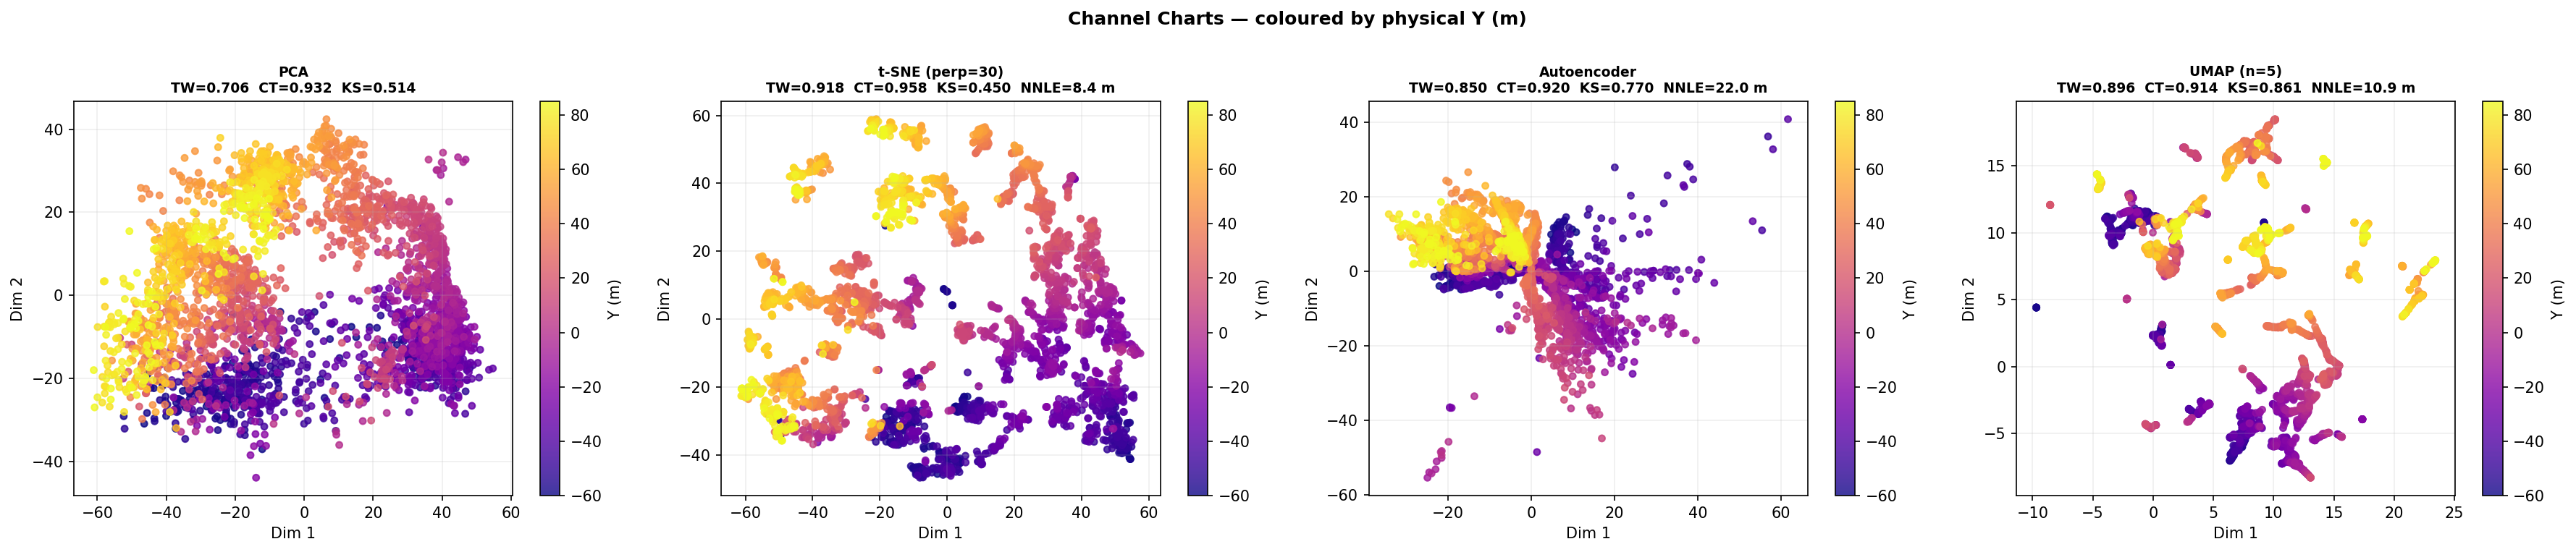
\includegraphics[width=\textwidth]{pictures/04_channel_charting/channel_charts_coloured_y.png}
  \caption{Same four charts coloured by the ground-truth $y$ coordinate.}
  \label{fig:cc_y}
\end{figure*}

\begin{figure*}[htbp]
  \centering
  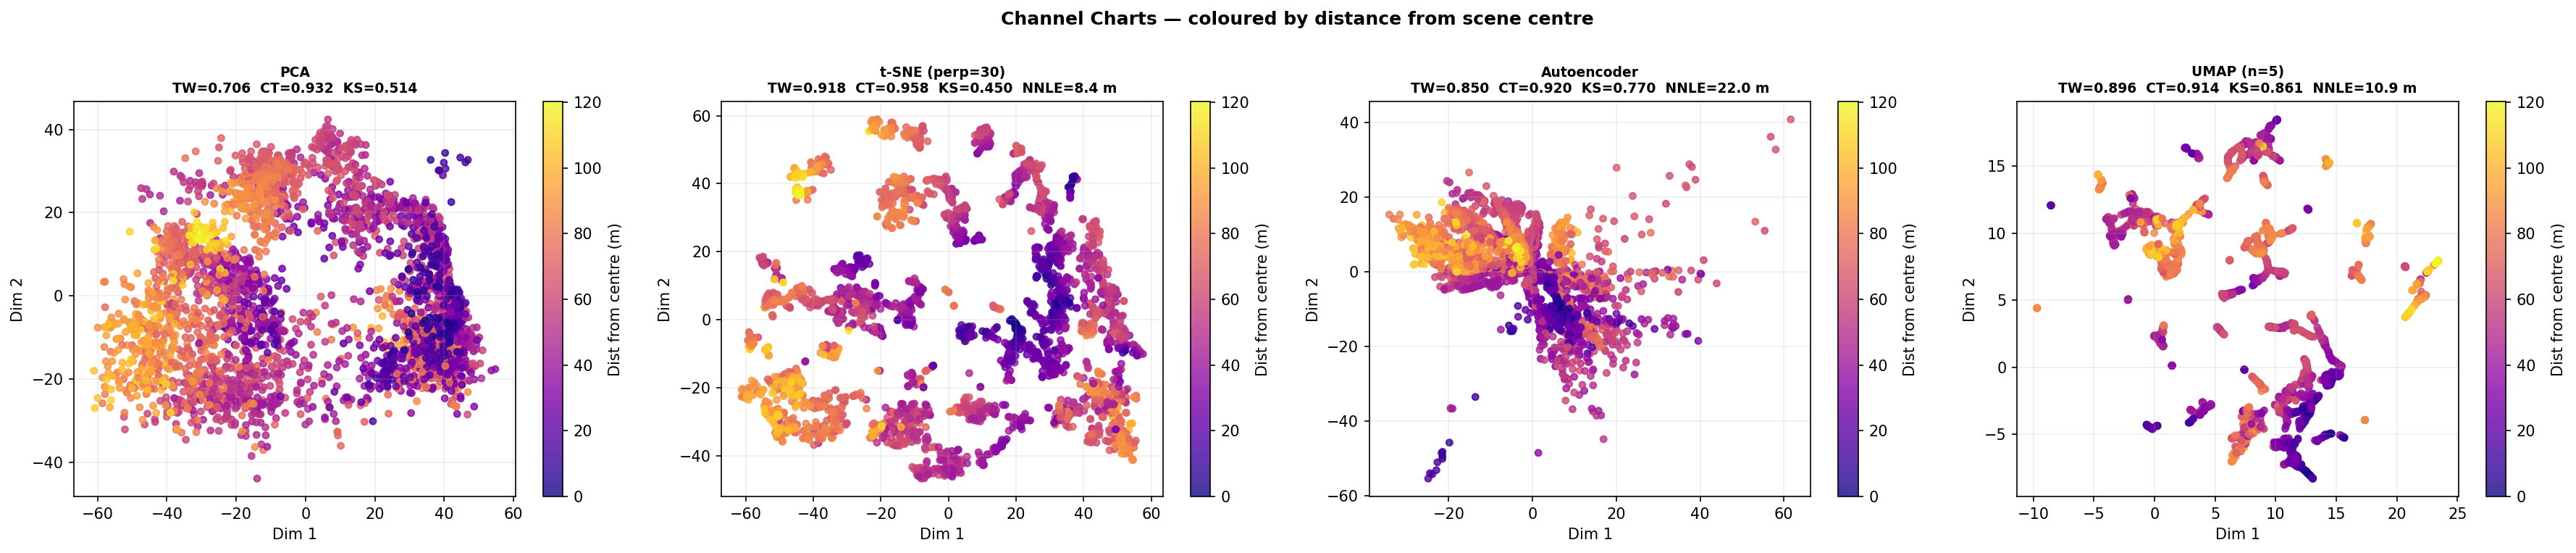
\includegraphics[width=\textwidth]{pictures/04_channel_charting/channel_charts_comparison.png}
  \caption{Charts coloured by distance from the scene centre.  t-SNE and
           UMAP produce the most geometrically consistent charts, PCA the
           most scale-faithful but topologically compressed one.}
  \label{fig:cc_comparison}
\end{figure*}

\begin{figure}[htbp]
  \centering
  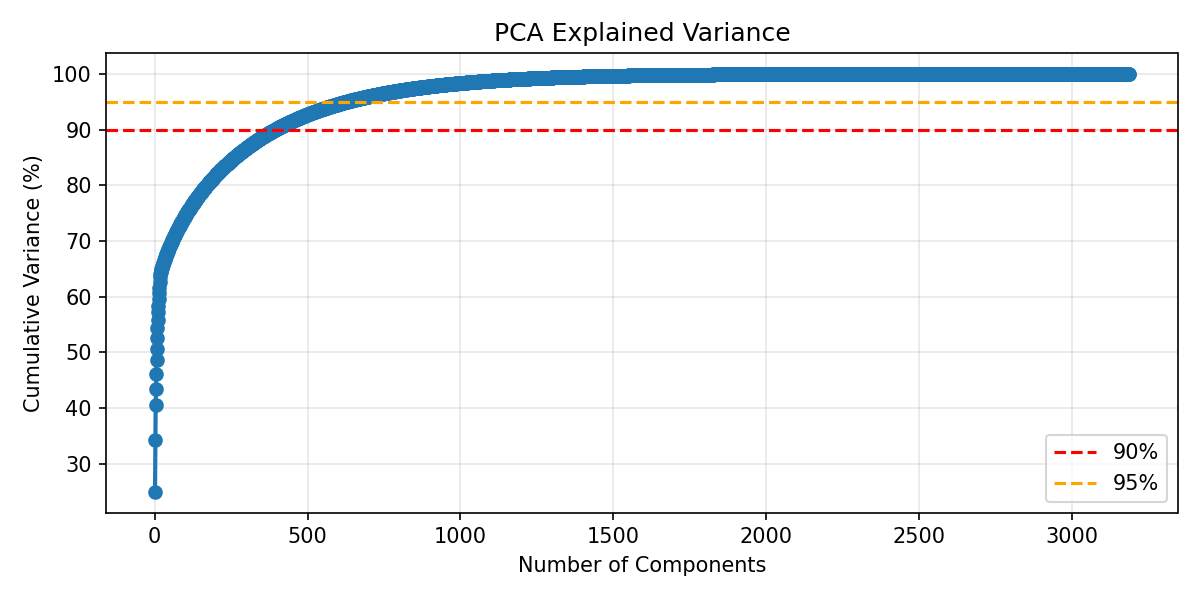
\includegraphics[width=\columnwidth]{pictures/04_channel_charting/pca_explained_variance.png}
  \caption{Cumulative explained variance of the PCA basis.  The first
           50 principal components, used as input to t-SNE and UMAP,
           capture the bulk of the fingerprint variance.}
  \label{fig:cc_pca}
\end{figure}

\subsection{Parameter Sensitivity}

Because t-SNE and UMAP are strongly sensitive to their local
neighbourhood parameters, both were swept on the same fingerprint matrix
(Table~\ref{tab:cc_sweep}).
t-SNE is relatively flat in TW for
$\text{perplexity}\in[15,50]$ but its KS score is minimised at
$\text{perplexity}=30$. Minum distance paramerter was set to 0.01 and 
metric was set to cosine for UMAP runs 
UMAP's $n_{\mathrm{neighbors}}$ trades neighbourhood TW against global
KS; the $n=5$ setting gives the best TW at the cost of a larger KS, and
is the working point reported in Table~\ref{tab:cc_metrics}.

\begin{table}[htbp]
\caption{Parameter sensitivity for t-SNE and UMAP}
\label{tab:cc_sweep}
\centering
\begin{tabular}{llrr}
\toprule
Method & Parameter                          & TW    & KS    \\
\midrule
t-SNE  & perplexity $= 5$                    & 0.906 & 0.459 \\
t-SNE  & perplexity $= 15$                   & 0.916 & 0.417 \\
t-SNE  & perplexity $= 30$                   & \textbf{0.918} & \textbf{0.450} \\
t-SNE  & perplexity $= 50$                   & 0.917 & 0.535 \\
\midrule
UMAP   & $n_{\mathrm{neighbors}} = 5$        & \textbf{0.896} & 0.861 \\
UMAP   & $n_{\mathrm{neighbors}} = 10$       & 0.896 & 0.870 \\
UMAP   & $n_{\mathrm{neighbors}} = 20$       & 0.895 & 0.884 \\
UMAP   & $n_{\mathrm{neighbors}} = 30$       & 0.891 & 0.898 \\
\bottomrule
\end{tabular}
\end{table}

\subsection{t-SNE and UMAP on MATLAB}

Table~\ref{tab:cc_sweep_matlab} summarises the performance of t-SNE and UMAP matlab
 implementations for different parameters and number of neighbors.  
 
 t-SNE perplexities are shown in Fig \ref{fig:cc_tsne_matlab}.



\begin{table}[htbp]
\caption{Parameter sensitivity for t-SNE and UMAP}
\label{tab:cc_sweep_matlab}
\centering
\begin{tabular}{llrrr}
\toprule
Method & Parameter                          & TW    & CT    &   KS\\
\midrule
t-SNE  & perplexity $= 30$                    & 0.8649 & 0.9024 & 0.4953\\
t-SNE  & perplexity $= 50$                    & 0.8515 &  0.9010 & 0.4847\\
t-SNE  & perplexity $= 100$                   & 0.8706 & 0.9007 & 0.4992\\
\midrule
UMAP   & $n_{\mathrm{neighbors}} = 5$        & 0.8618 & 0.8949 & 0.7451\\
UMAP   & $n_{\mathrm{neighbors}} = 10$       & 0.8769  & 0.8967 & 0.5509\\
UMAP   & $n_{\mathrm{neighbors}} = 20$       & 0.8771 & 0.8973 & 0.5771\\
UMAP   & $n_{\mathrm{neighbors}} = 30$       & 0.8472 & 0.8955 & 0.8049\\
\bottomrule
\end{tabular}
\end{table}


\begin{figure*}[htbp]
  \centering
  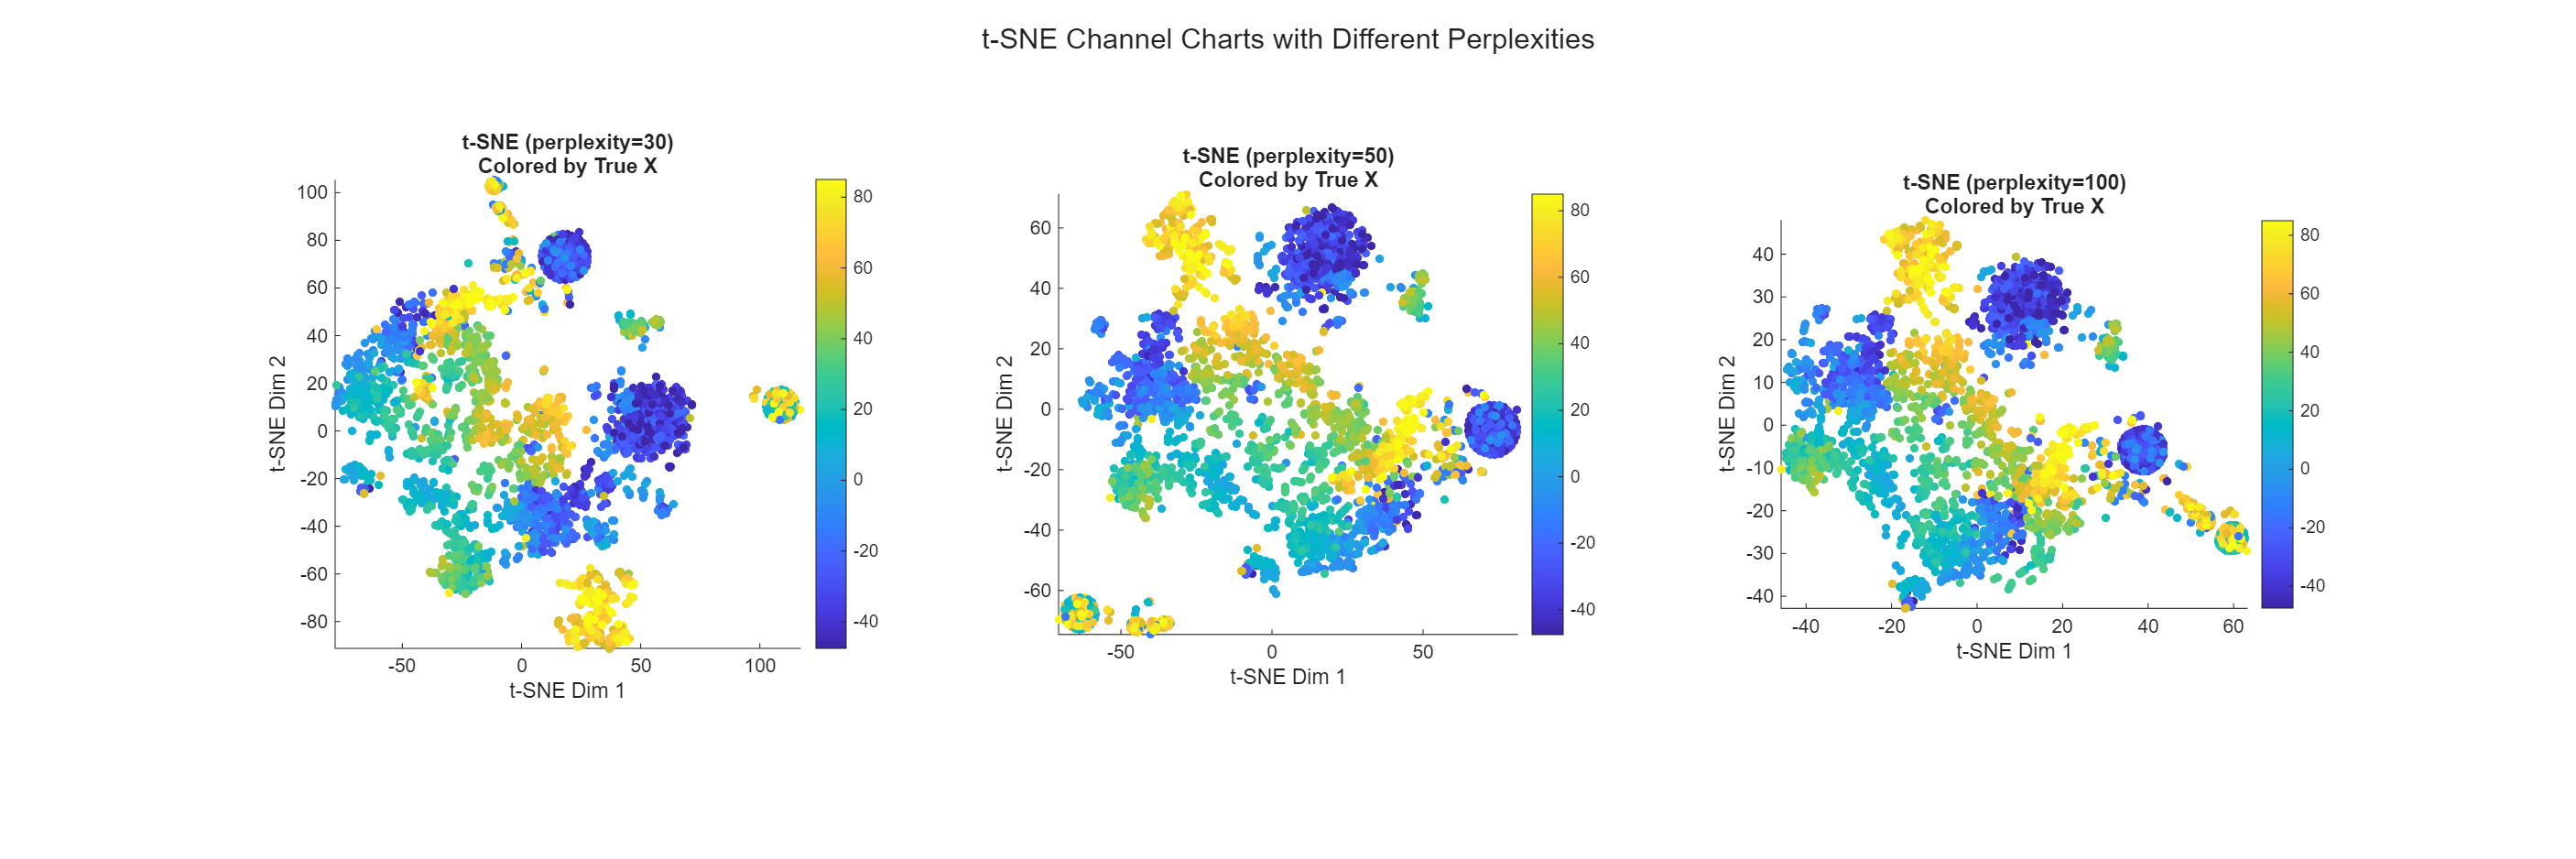
\includegraphics[width=\textwidth]{pictures/TSNE_perplexities.png}
  \caption{t-SNE channel charts for different perplexity values.}
  \label{fig:cc_tsne_matlab}
\end{figure*}



\subsection{Discussion}

t-SNE at perplexity $30$ is the best method on every metric, with
$\text{TW}=0.918$, $\text{CT}=0.958$, and a nearest-neighbour localisation
error of $8.35\,\text{m}$, which is on par with the best supervised
regressor of Section~\ref{sec:localization} despite using no UE labels.
UMAP trades a little TW/CT against substantially worse KS, which is the
expected behaviour of a method optimised for local topology preservation.
The autoencoder is the weakest of the four on KS ($0.77$) and NNLE
($22\,\text{m}$): its MSE reconstruction objective does not explicitly
encourage metric preservation in the latent space, and the small number
of training fingerprints ($N=3\,186$) is insufficient for a deep latent
model.
PCA, as expected, provides a cheap but strongly non-metric baseline
(high CT but poor TW and KS): variance directions in the CSI space are
not aligned with geographic axes.

Practical improvements fall into three categories:
\begin{enumerate}
  \item \emph{Richer fingerprints} --- include per-path AoA/AoD (already
        available in the HDF5 dataset) and stack CSI from all BSs
        equally rather than the current flat feature vector.
  \item \emph{Structure-aware losses} --- replacing the plain MSE
        autoencoder with a triplet or Siamese training
        objective~\cite{lei2019siamese_cc} would force the latent space
        to preserve neighbourhood relationships directly.
  \item \emph{Scene size} --- enlarging the UE grid (reducing
        \texttt{GRID\_SPACING}) increases the density of the fingerprint
        library and reduces the sampling noise in the DR metrics.
\end{enumerate}

\subsection{MATLAB Pipeline Cross-Check to Python environment}
\label{sec:matlab_channel_charting}

The same four DR methods were also applied to the MATLAB-derived
 fingerprints (Section~\ref{sec:matlab_dataset}),
with $N=3\,069$ UE positions and a much narrower feature vector
($D_f = 63$: AoA+RSS+Dly+Rch only).
Table~\ref{tab:cc_matlab} summarises the results.

\begin{table}[htbp]
\caption{Channel-charting metrics on the MATLAB tommiScene corpus ($N = 3\,069$, $D_f = 63$).  Best value per column in \textbf{bold}.}
\label{tab:cc_matlab}
\centering
\begin{tabular}{lrrrr}
\toprule
Method              & TW ($\uparrow$) & CT ($\uparrow$) & KS ($\downarrow$) & NNLE (m, $\downarrow$) \\
\midrule
PCA                 & 0.613            & 0.830            & 0.523              & n/a \\
t-SNE (perp.\ = 5)  & \textbf{0.975}   & \textbf{0.945}   & 6.828              & \textbf{19.46} \\
Autoencoder         & 0.754            & 0.885            & 0.478              & 40.02 \\
UMAP ($n=5$)        & 0.954            & 0.936            & \textbf{0.397}     & 22.04 \\
\bottomrule
\end{tabular}
\end{table}

Qualitatively the same ranking emerges as on the Sionna corpus: t-SNE
gives the best neighbourhood-preservation (highest TW, lowest NNLE),
UMAP is the best \emph{scale-faithful} chart (lowest KS), PCA is the
weak linear baseline, and the autoencoder struggles with the small
feature vector.
The absolute NNLE is worse than on the Sionna corpus
($19.46\,\text{m}$ vs.\ $8.35\,\text{m}$), consistent with the coarser
localization result in Section~\ref{sec:matlab_localization}: fewer
effective features means less neighbourhood information for the DR
method to exploit.
The MATLAB t-SNE KS value of $6.83$ is unusually large, reflecting the
fact that t-SNE's output is not globally scale-preserving; UMAP or PCA
are the right choices when absolute distance matters.



\section{Conclusion and Future Work}
\label{sec:conclusion}

This paper presented an end-to-end methodology for wireless channel dataset
generation, fingerprint localization, and channel charting on the Otaniemi
campus.
A cropped $132\,\text{m}\times 147\,\text{m}$ sub-region of the Aalto
School of Electrical Engineering was instrumented with nine rooftop
5G NR~Band~n78 sites ($f_c = 3.6\,\text{GHz}$,
$4\times4$ antennas per BS), and a $2.5\,\text{m}$ UE grid with
3\,069 valid positions.
The wireless channel dataset was generated using MATLAB's Ray Tracing
toolbox with configurable path-tracing parameters (reflections, diffractions, frequency)
to produce physically realistic multipath channel characteristics for both
localization and channel-charting applications.

The resulting fingerprint matrices were used in two complementary ways.
A $3\,069 \times 63$ MATLAB-derived fingerprint matrix (with AoA, RSS, delay, and LOS features)
generated from MATLAB ray-tracing and processed in Python served as an independent
validation dataset.
For \emph{fingerprint localization} (Section~\ref{sec:localization}),
six estimators were benchmarked on the MATLAB-derived dataset under a 70\,\%/30\,\% train/test split;
wKNN with coarse-to-fine refinement and MLP regression reached comparable performance
($\text{MAE} \approx 18\,\text{m}$), demonstrating the robustness of fingerprinting
across different ray-tracing implementations and feature representations.
A classification head on the same grid failed because the cell count
exceeded the number of training samples --- a clear demonstration of
why regression is preferable to classification for dense grids.
For \emph{channel charting} (Section~\ref{sec:channel_charting}), four
DR methods (PCA, t-SNE, autoencoder, UMAP) were scored with
TW/CT/KS/NNLE on both the Otaniemi\_small and MATLAB-derived datasets;
t-SNE produced strong unsupervised maps on both datasets, with
$\text{TW}=0.918$, $\text{CT}=0.958$ on Otaniemi\_small and $\text{TW}=0.975$, $\text{CT}=0.945$
on the MATLAB-derived dataset --- comparable to the best supervised regressor without
using any UE labels.

Overall the Otaniemi campus testbed, validated through independent MATLAB ray-tracing
simulation, is a useful mid-scale environment: large enough to produce
non-trivial NLOS structure that stresses both the localizer and the chart, yet tractable
for CPU-only processing.
The main limitations observed were (i) the dominant geometric ambiguity
in the shadow regions behind large facades, which inflates the tail of
the localization error CDF across both datasets; (ii) the reduced feature
dimensionality in the MATLAB-derived feature vector (63 dimensions: AoA, RSS, delay, LOS)
compared to full CSI fingerprints, which limits performance for data-hungry models;
and (iii) the limited number of grid samples for deep learning models such
as the plain MSE autoencoder.

\subsection*{Future Work}

Several follow-on directions are natural.
First, the fingerprint vector currently uses only amplitude-domain
features; incorporating the per-path AoA/AoD angles already available in
the HDF5 dataset is expected to sharpen both the localizer and the
chart~\cite{hoydis2023sionna_rt,3gpp_nr_channel}.
Second, replacing the plain-MSE autoencoder with a
Siamese/triplet-loss AE~\cite{lei2019siamese_cc} would give the latent
space an explicit metric-preservation objective and should close most of
the gap to t-SNE.
Third, extending the scene size --- by reverting to the full 77-building
Otaniemi model once a GPU host is available --- would capture more
propagation diversity and enable multi-point channel charting across
adjacent cells.
Fourth, a semi-supervised channel-chart formulation, in which a small
subset of labelled anchors regularises the latent space, is a direct
avenue for the extra-credit item in the course
assignment~\cite{studer2018channel_charting}.
Finally, closing the loop by using the chart as an input to a
beam-management or handover policy would demonstrate the practical
utility of the learned radio-space embedding for real 5G/beyond-5G
systems~\cite{sionna2022}.


\appendix
\section*{Appendix A: Detailed Channel Analysis Report}
\label{app:analysis_report}

A comprehensive analysis of the wireless channel characteristics for the
Otaniemi\_small scenario is available in the supplementary analysis report
(\texttt{Otaniemi\_small\_analysis\_report.pdf}). This report includes:

\begin{itemize}
  \item \textbf{Dataset Generation:} Detailed visualization of the geographic
        scene, base-station layout, UE grid, and simulation parameters.
  \item \textbf{Ray-Tracing Comparison:} Multipath statistics including
        channel impulse responses, path-level delay spread, angular spread
        analysis, and head-to-head comparison between Sionna\,RT and the
        independent MATLAB ray-tracing validation dataset.
  \item \textbf{Fingerprint Features:} Comprehensive coverage of CSI
        feature extraction, feature-ablation study results, and identification
        of the dominant feature families for localization.
  \item \textbf{Channel Charting:} Visualization of the channel state space
        using multiple dimensionality-reduction methods and spatial
        trustworthiness metrics.
\end{itemize}

The supporting data, intermediate results, and detailed figures referenced
in this paper are archived in the project repository and may be reproduced
by running the analysis pipeline on the Otaniemi OSM building model with
the documented simulation parameters.


\section*{Acknowledgment}
The authors would like to thank the course lecturer and teaching assistants
for supporting this project, and the Aalto University School of Electrical
Engineering for providing computational resources.

\bibliographystyle{IEEEtran}
\nocite{*}
\bibliography{references}

\end{document}
